\documentclass[12pt,a4paper]{report}

% ---------- Packages ----------
\usepackage[utf8]{inputenc}
\usepackage[T1]{fontenc}
\usepackage[margin=2.5cm]{geometry}
\usepackage{amsmath,amssymb}
\usepackage{graphicx}
\usepackage{booktabs,multirow,array}
\usepackage{subcaption}
\usepackage{listings}
\usepackage{xcolor}
\usepackage{tikz}
\usepackage{fancyhdr}
\usepackage{hyperref}

% ---------- Header and footer ----------
\setlength{\headheight}{15pt}
\pagestyle{fancy}
\fancyhf{}
\fancyhead[L]{LaTeX Examples}
\fancyhead[R]{\leftmark}
\fancyfoot[C]{\thepage}

% ---------- Custom commands ----------
\newcommand{\tool}[1]{\textbf{\textcolor{blue}{#1}}}
\newcommand{\vect}[1]{\mathbf{#1}}

% ---------- Code listing style ----------
\lstset{basicstyle=\ttfamily\small, frame=single,
        numbers=left, breaklines=true, keywordstyle=\color{blue}}

\title{\LaTeX{} Documentation Examples}
\author{Suraj Pathak\\MNIT Jaipur}
\date{\today}

\begin{document}
\maketitle
\begin{abstract}
This document demonstrates the main features of \LaTeX{}: structure,
text formatting, lists, mathematics, tables, figures, references,
page layout, custom commands and code listings.
\end{abstract}
\tableofcontents

\chapter{Structure and Text}

\section{Document structure}
A \LaTeX{} file has a \emph{preamble} (before \verb|\begin{document}|)
and a \emph{body}. Sectioning commands: \verb|\chapter|, \verb|\section|,
\verb|\subsection|, \verb|\subsubsection|, \verb|\paragraph|.

\subsection{A subsection}
Text of the subsection.

\subsubsection{A subsubsection}
Text of the subsubsection.

\section{Text formatting}
\textbf{Bold}, \textit{italic}, \underline{underline}, \texttt{typewriter},
\textsc{Small Caps}, \emph{emphasis}.

{\tiny tiny} {\small small} {\normalsize normal} {\large large}
{\Large Large} {\huge huge}

\begin{center}
Centered text
\end{center}
\begin{flushright}
Right-aligned text
\end{flushright}

Special characters must be escaped: \$ \% \& \# \_ \{ \} .

A new paragraph starts after a blank line.\\
This line starts after a forced line break.

\noindent No indentation here. \hspace{1cm} A horizontal gap.
\vspace{0.5cm}

% This is a comment and does not appear in the output.
\newpage

\chapter{Lists and Mathematics}

\section{Lists}
\begin{itemize}
  \item First item
  \item Second item
  \begin{itemize}
    \item Nested item
  \end{itemize}
\end{itemize}

\begin{enumerate}
  \item Step one
  \item Step two
\end{enumerate}

\begin{description}
  \item[Git] Version control system.
  \item[GitHub] Hosting platform for Git repositories.
\end{description}

\section{Mathematics}
Inline math: $E = mc^2$ and $\alpha + \beta = \gamma$.

Display math with numbering:
\begin{equation}
  x = \frac{-b \pm \sqrt{b^2 - 4ac}}{2a}
  \label{eq:quad}
\end{equation}
Equation~\ref{eq:quad} is the quadratic formula.

Unnumbered display: \[ \sum_{i=1}^{n} i = \frac{n(n+1)}{2} \]

Aligned equations:
\begin{align}
  (a+b)^2 &= a^2 + 2ab + b^2 \\
  (a-b)^2 &= a^2 - 2ab + b^2
\end{align}

Integral and limit:
\[ \int_{0}^{\infty} e^{-x}\,dx = 1, \qquad \lim_{x \to 0}\frac{\sin x}{x} = 1 \]

Matrix:
\[
A = \begin{bmatrix} 1 & 2 \\ 3 & 4 \end{bmatrix},
\qquad \vect{v} = \begin{pmatrix} x \\ y \end{pmatrix}
\]

Piecewise function:
\[
f(x) = \begin{cases}
  x^2 & x \ge 0 \\
  -x  & x < 0
\end{cases}
\]

\chapter{Tables and Figures}

\section{Tables}
\begin{table}[h]
\centering
\begin{tabular}{|l|c|r|}
\hline
\textbf{Left} & \textbf{Center} & \textbf{Right} \\ \hline
A & B & C \\ \hline
Long text & 12 & 3.14 \\ \hline
\end{tabular}
\caption{A basic table}
\label{tab:basic}
\end{table}

Professional style with \texttt{booktabs}, \texttt{multicolumn} and \texttt{multirow}:
\begin{table}[h]
\centering
\begin{tabular}{llr}
\toprule
\multicolumn{2}{c}{\textbf{Tool}} & \textbf{Year} \\
\midrule
\multirow{2}{*}{Version control} & Git & 2005 \\
                                 & SVN & 2000 \\
Documentation & Doxygen & 1997 \\
\bottomrule
\end{tabular}
\caption{A table using booktabs}
\label{tab:booktabs}
\end{table}
Tables~\ref{tab:basic} and~\ref{tab:booktabs} show two table styles.

\section{Figures}
\LaTeX{} can draw graphics itself using TikZ. A figure with a caption:
\begin{figure}[h]
\centering
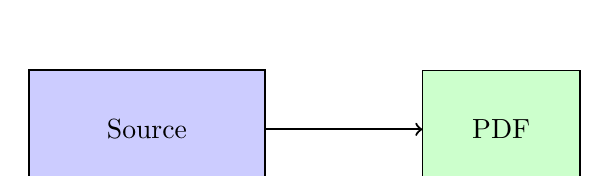
\begin{tikzpicture}
  \draw[thick,fill=blue!20] (0,0) rectangle (3,1.5);
  \draw[thick,->] (3,0.75) -- (5,0.75);
  \node at (1.5,0.75) {Source};
  \node[draw,fill=green!20,minimum width=2cm,minimum height=1.5cm] at (6,0.75) {PDF};
\end{tikzpicture}
\caption{A simple TikZ diagram}
\label{fig:tikz}
\end{figure}
See Figure~\ref{fig:tikz}.

To include an image file use
\verb|\includegraphics[width=0.6\textwidth]{image.png}| (needs \texttt{graphicx}).

\subsection{Subfigures}
\begin{figure}[h]
\centering
\begin{subfigure}{0.4\textwidth}
  \centering
  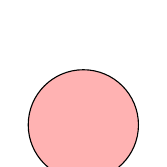
\begin{tikzpicture}\draw[fill=red!30] (0,0) circle (0.7);\end{tikzpicture}
  \caption{Circle}
\end{subfigure}
\begin{subfigure}{0.4\textwidth}
  \centering
  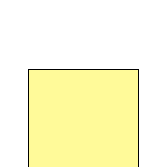
\begin{tikzpicture}\draw[fill=yellow!40] (0,0) rectangle (1.4,1.4);\end{tikzpicture}
  \caption{Square}
\end{subfigure}
\caption{Two subfigures}
\end{figure}

\chapter{References, Code and Commands}

\section{Cross-references and citations}
Use \verb|\label| and \verb|\ref| for cross-references:
Chapter~\ref{ch:custom} is on custom commands.
Citations use BibTeX: the standard references are \cite{lamport1994,knuth1984},
and information theory started with \cite{shannon1948}.
Hyperlinks: \url{https://www.latex-project.org/} or
\href{https://www.overleaf.com}{Overleaf}.
Footnote example.\footnote{A footnote appears at the bottom of the page.}

\section{Code listings}
\begin{lstlisting}[language=Python, caption={A Python listing}]
def add(a, b):
    return a + b

print(add(2, 3))
\end{lstlisting}

Inline code: \lstinline|git commit -m "message"|.

\section{Custom commands}
\label{ch:custom}
Commands defined in the preamble: \tool{Git}, \tool{LaTeX}, and a vector $\vect{x}$.
Syntax: \verb|\newcommand{\name}[num args]{definition}|.


\bibliographystyle{plain}
\bibliography{references}

\appendix
\chapter{Appendix Example}
Appendices use \verb|\appendix| and then \verb|\chapter| or \verb|\section|.

\end{document}
